\section{Introduction}
\label{sec:introduction}

Numerous astronomical observations suggest the existence of a substance that permeates the universe, and which appears to only interact significantly with ordinary matter via gravity. Attempts to directly observe it have been unsuccessful, but this mysterious ``dark matter'' is estimated to make up over a quarter of the total mass-energy in the universe. It remains an open possibility that dark matter interacts with ordinary matter by other means besides gravitation, and implies dark matter may be produced directly by the LHC. If produced, dark matter particles are practically invisible to the detector and therefore manifest as missing energy in the event. This document describes a search for dark matter produced in association with $\ttbar$ in $13\:\TeV$ $\PP$ collisions with the CMS detector.

The simplest and most compelling model for dark matter production with $\ttbar$ proposes a spin-$0$ interaction between dark matter (DM) and Standard Model (SM) particles. At leading order, the process is gluon-induced and a $\ttbar$ pair is produced with a pair of DM fermions. The coupling to SM particles is taken to be Yukawa, and hence is proportional to mass and favoring $\Top$ quarks. The DM fermions can be Dirac or Majorana in nature with the difference being a factor of two in the cross section; they are taken to be Dirac fermions in the signal samples used in this analysis.

\subsection{Effective Field Theory}
\label{subsec:intro_eft}
The most basic theory of $\ttbar+$DM production describes a contact interaction between DM and SM particles. This model is valid under a few assumptions, the main one being that the exchanged mediator particle is too heavy to be produced by collisions. This theory is typically called the effective field theory (EFT) and is characterized by the mass of the DM fermion, $M_\chi$, and the interaction mass scale, $M_{*} = M_{\Phi}/\sqrt{g_q g_\chi}$, where $M_{\Phi}$ is the mass of the mediator, $g_q$ is the coupling of the mediator and SM particle, and $g_\chi$ is the coupling of the mediator and DM particle. The production cross section of $\ttbar+$DM is then proportional to $m_t^2/M_*^6$, where $m_t$ is the $\Top$-quark mass. Searches for $\ttbar+$DM in Run-1 were interpreted in the context of EFT.

\subsection{Simplified Model}
\label{subsec:intro_sms}
The EFT is limited in the range of dynamics and kinematics it can describe. A \emph{simplified model} for DM production can be constructed by relaxing the assumption of contact interaction and involving the mediator explicitly in the theory. The simplified model is then characterized by four parameters: $M_\Phi$, $M_\chi$, $g_q$, and $g_\phi$. A minimal set of benchmark simplified model points have been decided upon from the ATLAS-CMS Dark Matter Forum. The benchmarks consists of representative points to cover all the interesting kinematic features in phase space that would be relevant with $O(10\:\ifb)$ of integrated luminosity at $13\:\TeV$. The kinematics depend most strongly on $M_\Phi$ and $M_\chi$, while the couplings induce smaller or more subtle kinematic effects, therefore the benchmarks are a set of $\left(M_\chi,\,M_\Phi\right)$ combinations with couplings fixed at $g_q=g_\chi=1$. The benchmark points are listed in Table~\ref{tab:dmf}.

\begin{figure}[!htbp]
\begin{center}
  \subfigure[]{\label{subfig:eft}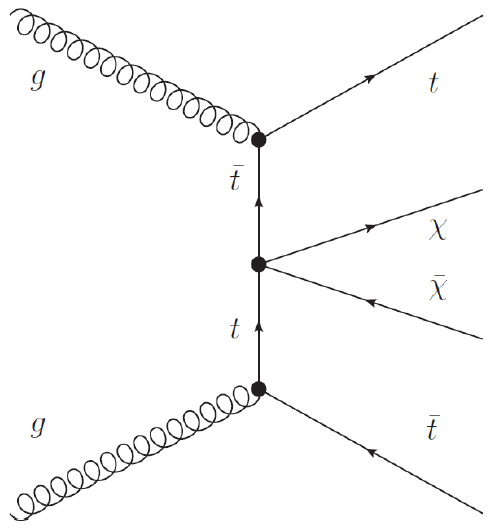
\includegraphics[width=0.30\textwidth]{figures/eft.png}}
  \hspace{2cm}
  \subfigure[]{\label{subfig:sms}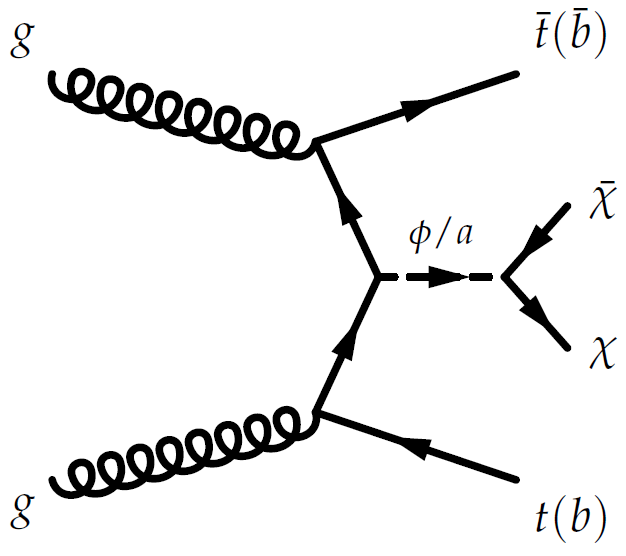
\includegraphics[width=0.35\textwidth]{figures/sms.png}}
  \caption{Diagrams for \subref{subfig:eft} effective field theory and \subref{subfig:sms} and simplified model.}
  \label{fig:ttdm_diagrams}
\end{center}
\end{figure}

\begin{table}[!ht]
\centering
\begin{tabular}{|l|ccccccccc|}
\hline
  \multicolumn{1}{|c|}{$M_{\chi}$ ($\GeV$)} & \multicolumn{9}{|c|}{$M_{\mbox{\scriptsize{med}}}$ ($\GeV$)} \\
\hline
  $1$    & $10$ & $20$ & $50$ & $100$ & $200$ & $300$ & $500$ & $1000$ & $10000$ \\
  $10$   & $10$ & $15$ & $50$ & $100$ &       &       &       &        & $10000$ \\
  $50$   & $10$ &      & $50$ & $95$  & $200$ & $300$ &       &        & $10000$ \\
  $150$  & $10$ &      &      &       & $200$ & $295$ & $500$ & $1000$ & $10000$ \\
  $500$  & $10$ &      &      &       &       &       & $500$ & $995$  & $10000$ \\
  $1000$ & $10$ &      &      &       &       &       &       & $1000$ & $10000$ \\
\hline
\end{tabular}
\caption{Simplified model benchmarks for $s$-channel simplified models with spin-$0$ mediators decaying to Dirac DM fermions.}
\label{tab:dmf}
\end{table}

\subsection{Analysis Strategy Overview}
\label{subsec:intro_anastrat}
This analysis approach is a categorized \met-shape fit, where the categories are formed based on resolved top tagging variables. As a reference, we also pursue a simple Poisson counting analysis with both categorized and uncategorized cases.

